%%
%% This is file `example_DarkConsole.tex',
%% generated with the docstrip utility.
%%
%% The original source files were:
%%
%% examples_kmbeamer.dtx  (with options: `DarkConsole')
%% Copyright (c) 2011-2013 Kazuki Maeda <kmaeda@users.sourceforge.jp>
%% 
%% Distributable under the MIT License:
%% http://www.opensource.org/licenses/mit-license.php
%% 

%%% もし pdfTeX や LuaTeX を使うなら dvipdfmx オプションを外す.
% \documentclass[dvipdfmx]{beamer}

% Modified by LianTze Lim to work with fontspec/xelatex
\documentclass{beamer}
\usepackage{mathspec}
\usepackage{xeCJK}
\setCJKmainfont{IPAPMincho}
\setCJKsansfont{IPAGothic}
\setCJKmonofont{IPAGothic}

% You can set fonts for Latin script here
\setmainfont{FreeSerif}
\setsansfont{FreeSans}
\setmonofont{Latin Modern Mono}
\setcounter{secnumdepth}{5}
\setcounter{tocdepth}{5}
\usetheme{DarkConsole}
\usepackage{graphicx} 
\usepackage{auto-pst-pdf} 

%%% もし pTeX + dvipdfmx を使うならば以下のどちらかを環境に合わせてコメントアウト.
%% \AtBeginDvi{\special{pdf:tounicode EUC-UCS2}} % EUC の場合
%% \AtBeginDvi{\special{pdf:tounicode 90ms-RKSJ-UCS2}} % SJIS の場合

%%% もし LuaTeX で日本語を出力するなら以下をコメントアウト.
%% \usefonttheme{luatexja}
%% \hypersetup{unicode}

%%% 日本語を使うなら以下を入れると定理環境中のフォントが立体になる.
%%% 欧文なら不要.
%%% LLT: Comment out this line if your presentation is in English or other European languages
\setbeamertemplate{theorems}[normal font]

\title{\texttt{mathematical description of} reactive sputtering in c}
\subtitle{based on berg model described in Journal of Vacuum Science \& Technology A: Vacuum, Surfaces, and Films 5, 202 (1987); doi:
10.1116/1.574104}
\author{sebastian matkovich\footnote{\texttt{e1026902@student.tuwien.ac.at}}}

\begin{document}

\begin{frame}
  \maketitle
\end{frame}

\begin{frame}{table of contents}
  \tableofcontents
\end{frame}

\section{equations}

\begin{frame}{steady state equations}


equation A5 for flux F of nitrogen molecules:
	  \begin{equation} F=\frac{p_{N}}{\sqrt{2k_{B}\pi TM}}  \end{equation}
equation A1' for target fractional coverage $\theta_{1}$:
	  \begin{equation} 2\alpha_{t}F(1-\theta_{1})-\frac{J}{e}S_{N}\theta_{1}=0  \end{equation}
equation A2' for chamber wall and substrate fractional coverage $\theta_{2}$:
	  \begin{equation} 2\alpha_{c}F(1-\theta_{2})+\frac{J}{e}S_{N}\theta_{1}\frac{A_{t}}{A_{c}}(1-\theta_{2})-\frac{J}{e}S_{M}(1-\theta_{1})\frac{A_{t}}{A_{c}}\theta_{2}=0 \end{equation}
equation A3 for flow to target:
	  \begin{equation} q_{t}=\alpha_{t}F(1-\theta_{1})A_{t}  \end{equation}
\end{frame}
\begin{frame}{steady state equations}
equation A4 for flow to surface area $A_{c}$ of the chamber:
	  \begin{equation} q_{c}=\alpha_{c}F(1-\theta_{2})A_{c}  \end{equation}
equation 2 for flow through pump:
		  \begin{equation} q_{p}=p_{N}S  \end{equation}
equation 1 for incoming reactive gas flow:
	  \begin{equation} q_{0}=q_{t}+q_{c}+q_{p}  \end{equation}
equation A6 for total sputtering rate Y:
	\begin{equation} R=\frac{J}{e}[S_{N}\theta_{1}+S_{M}(1-\theta_{1})] \end{equation}

\end{frame}
\section{algorithm}
\begin{frame}{algorithm}
	solve the equations by assuming a value for $p_{N}$. equations are already solved except A1' and A2', they can be written as:
	\begin{equation} \theta_{1}=\frac{1}{1+\frac{JS_{N}}{2e\alpha_{t}F}}  \end{equation}
		\begin{equation} \theta{2}=\frac{\frac{e}{J}2\alpha_{c}F\frac{A_{c}}{A_{t}}+S_N\theta{1}}{\frac{e}{J}2\alpha_{c}F\frac{A_{c}}{A_{t}}+S_N\theta{1}+S_{M}(1-\theta_{1})}  \end{equation}
			now assume a new (little higher) value for $p_{N}$
\end{frame}
\section{results}
\begin{frame}{results}
	for n=5000 iterations, $dp=10^{-6}$Pa pressurechange, $p_N=10^{-6}$Pa initial nitrogen partial pressure, T=300Kelvin, $M=4.651\cdot10^{-26}kg$ mass of nitrogen molecule, $S_{N}=0.3$ sputtering yield of compound by incoming argon ions, $J=14\frac{A}{m^{2}}$ current density of argon ions causing sputtering from target surface, $A_{t}=0.127m^{2}$ target surface, $A_{c}=1.27m^{2}$ exposed chamber surface, $S_{M}=1.5$ sputtering yield of elemental metalmaterial by incoming argon ions, $S=85\frac{l}{s}$ pumping speed, $\alpha_{t}=1$ sticking coefficient for nitrogen molecule to titanium target and $\alpha_{c}=1$ sticking coefficient for nitrogen molecule to titanium covered part $(1-\theta_{2})$ of chamber wall you can get these relationships: although for Y the lower part seems to be missing and for $P_N$ the higher part seems to be missing
\end{frame}
\begin{frame}{results}
	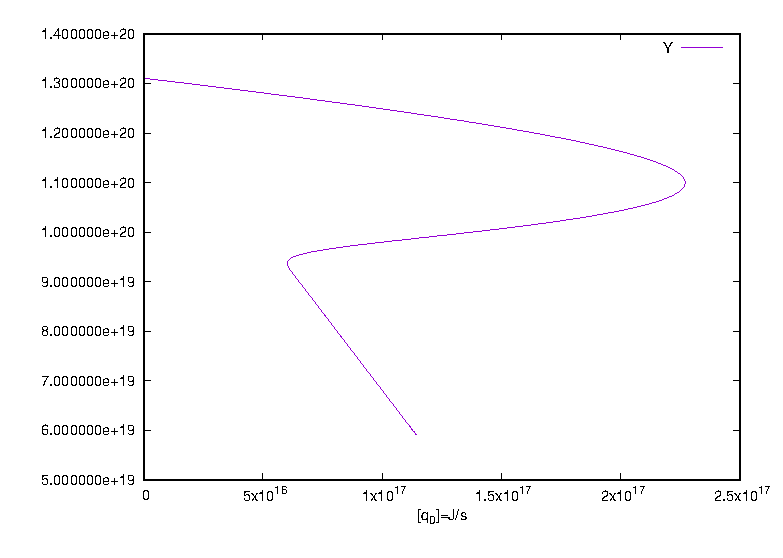
\includegraphics[width=2.3in]{YOverq_0.ps}
	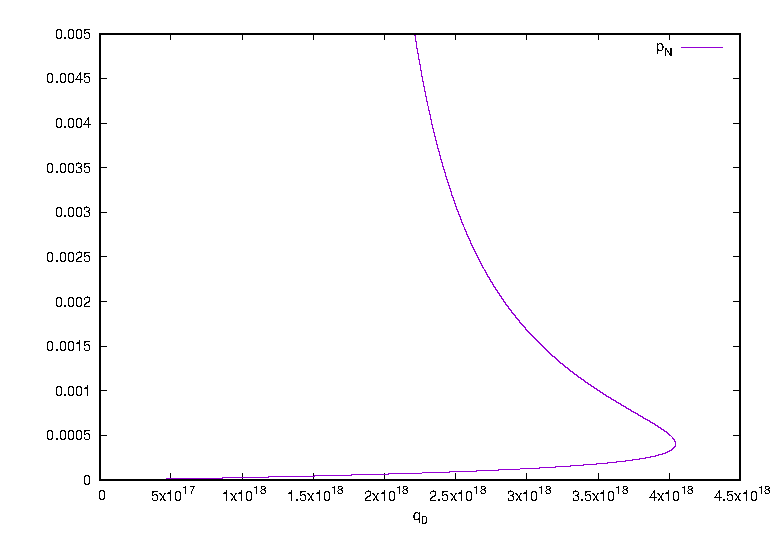
\includegraphics[width=2.3in]{p_NOverq_0.ps}

	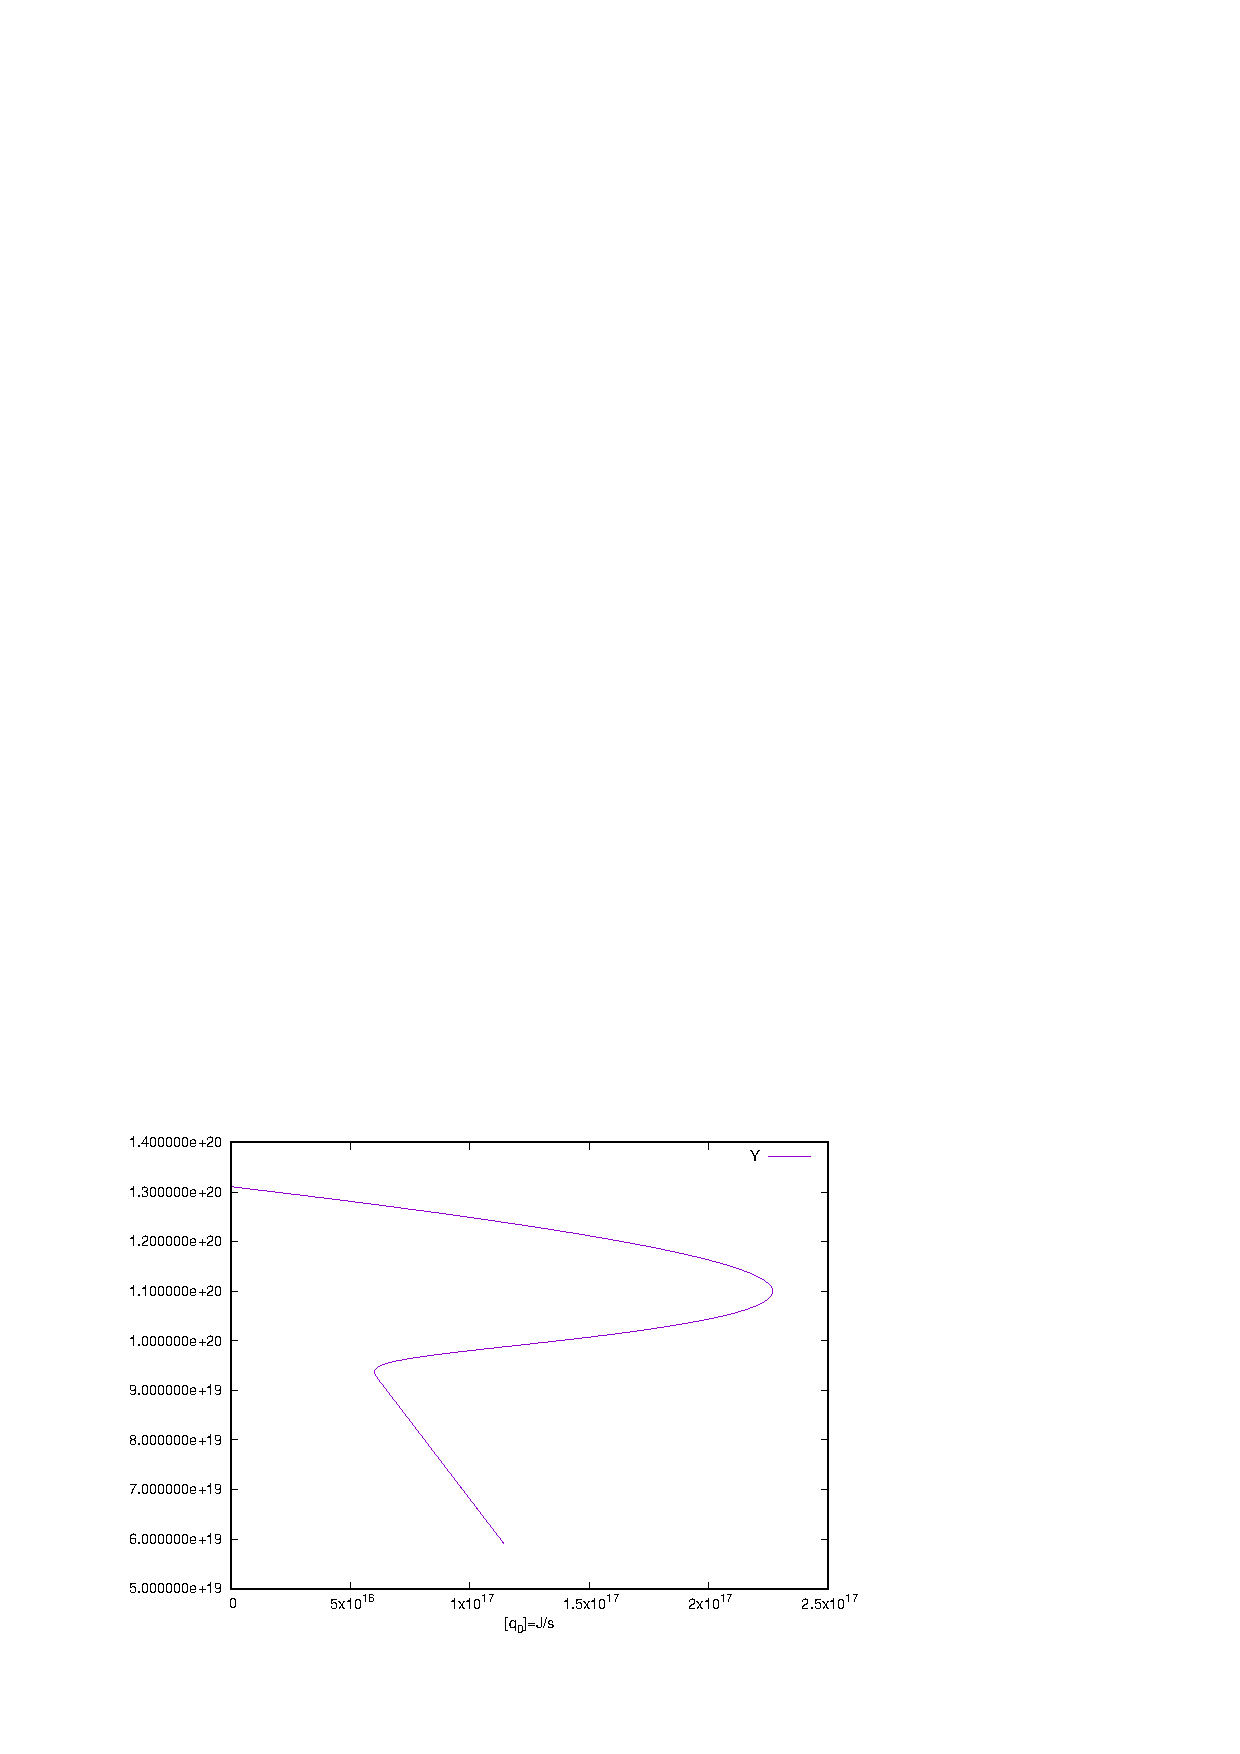
\includegraphics[width=2.3in]{YOverq_0.png}
	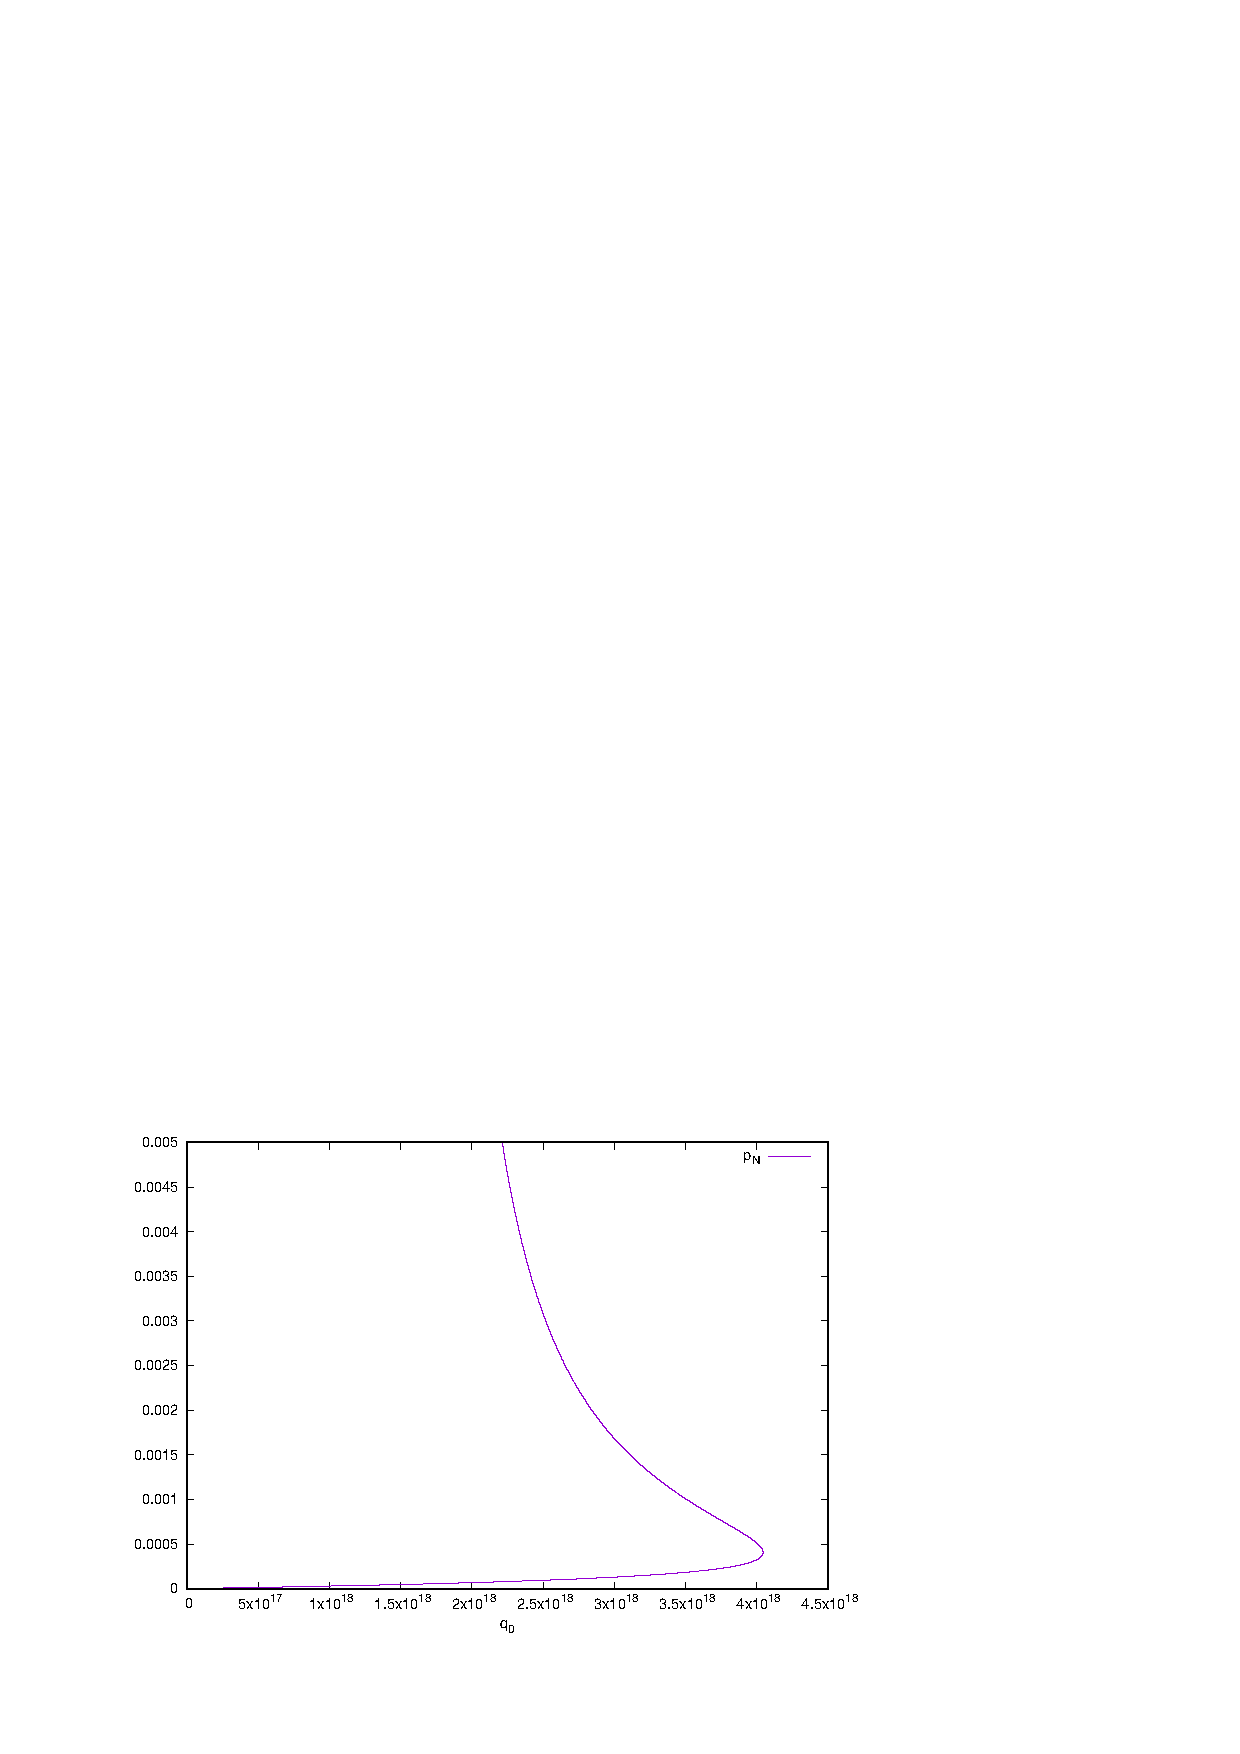
\includegraphics[width=2.3in]{p_NOverq_0.png}

\end{frame}
\end{document}
\endinput
%%
%% End of file `example_DarkConsole.tex'.

